\chapter{Implementacija}
\label{chp:Implementation}

U ovom poglavlju će biti opisana implementacija pratećeg projekta nazvanog \emph{Language Invariant Code Comparer} (skr. \emph{LICC}), pisanog u programskom jeziku C\# 8.0, koristeći \emph{.NET Core 3.1} radni okvir. C\# je izabran zbog lakoće implementacije velikih projekata i velike podrške paketa koji se mogu preuzeti, od kojih su korišćeni \emph{ANTLR Runtime} paket koji daje potrebne biblioteke za rad sa ANTLR generisanim parserima i \emph{Math.NET Symbolics} paket za rad sa simboličkim vrednostima. Rezultat je konzolna aplikacija koja može da generiše, serijalizuje ili prikaže opšti AST za dati izvorni k\^od, ali i da poredi takav AST sa drugim. Čitav projekat je dostupan u potpunosti na servisu GitHub na adresi \url{https://github.com/ivan-ristovic/LICC}.

Jedan od glavnih ciljeva aplikacije je modularnost i jednostavna proširivost. U tom duhu se, pored implementacije klasa potrebnih za predstavljanje opšte AST apstrakcije, pruža i interfejs za kreiranje adaptera koji će od proizvoljnog stabla parsiranja kreirati opšti AST. Kao primer, adapteri su kreirani za programske jezike C i Lua, a za primer potpune slobode u izboru gramatike je kreirana gramatika za pseudo-jezik i adapter za istu, što dozvoljava poređenje kodova sa specifikacijom datom u obliku pseudo-koda. Čitav projekat se sastoji od više komponenti, organizovanih po prostorima imena, od kojih su značajnije:
\begin{itemize}
    \item \texttt{LICC} --- Glavni program (korisnički interfejs) koji omogućava generisanje, prikaz, serijalizaciju i poređenje AST.
    \item \texttt{LICC.AST} ---Biblioteka klasa za rad sa opštom AST apstrakcijom.
    \item \texttt{LICC.Core} --- Upoređivač opštih AST --- konzolni izlaz.
    \item \texttt{LICC.Visualizer} --- Komponenta za vizualizaciju --- grafički prikaz AST.
    \item \texttt{LICC.Tests} --- Prateći testovi jedinica koda i integracioni testovi.
\end{itemize}

Čitava arhitektura data putem UML dijagrama komponenti se može videti na slici \ref{fig:ImplementationComponents}. Osim implementacije same aplikacije, svaki funkcionalni deo projekta prate i testovi jedinica koda, koji su povezani sa \emph{GitHub Actions} porškom za neprekidnu integraciju (engl. \emph{continuous integration}, srk. \emph{CI}). CI omogućava prevođenje izvornog koda nakon svake izmene kao i izvršavanje akcija nakon prevođenja kao što su testiranje ili generisanje predmeta za upotrebu (engl. \emph{artifacts}) koji predstavljaju rezultat procesa prevođenja i mogu se direktno isporučiti.

\begin{figure}[h!]
\centering
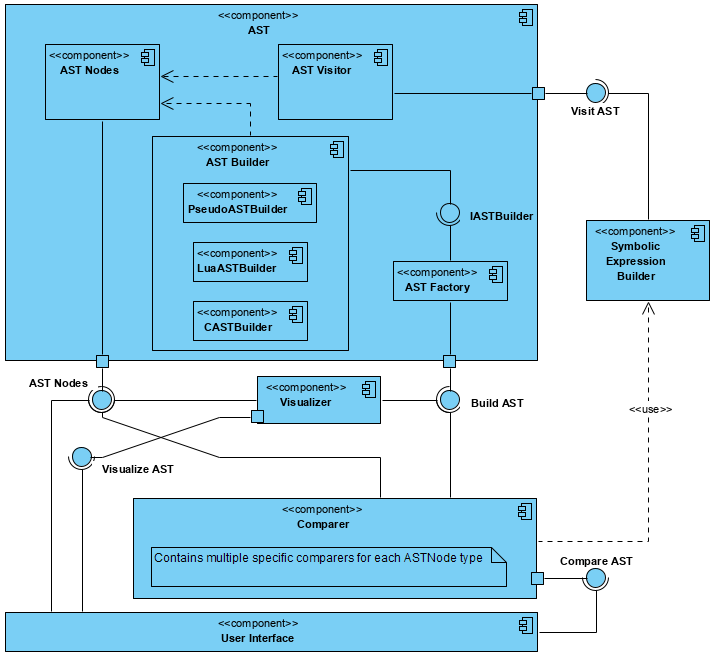
\includegraphics[scale=0.8]{images/uml/ComponentDiagram.png}
\caption{UML dijagram komponenti implementacije.}
\label{fig:ImplementationComponents}
\end{figure}


\section{Implementacija apstrakcije}
\label{sec:ImplementationMyAST}

Implementacija prati hijerarhije opisane u poglavlju \ref{chp:MyAST} kroz mehanizam nasleđivanja. Svaki tip čvora je implementiran kao zasebna klasa koja nasleđuje apstraktnu klasu \texttt{ASTNode}. Dijagram klasa koje nasleđuju klasu \texttt{ASTNode} se može videti na slikama \ref{fig:UMLASTNode1} i \ref{fig:UMLASTNode2}. Pored implementacije klasa koje predstavljaju AST čvorove, kreiran je i javno dostupni interfejs za obilazak AST putem obrazca posetilac u implementaciji korišćen za kreiranja graditelja simboličkog izraza od AST koji predstavlja izraz kao i evaluatora takvog AST.

\begin{figure}[h!]
\centering
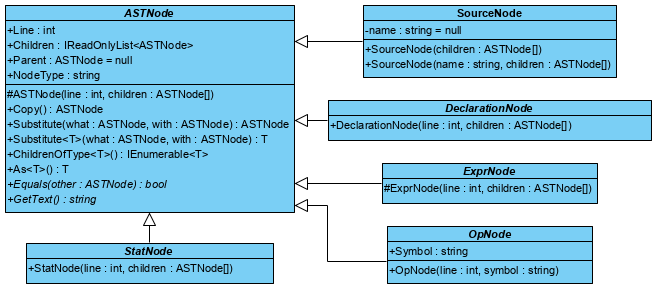
\includegraphics[scale=0.7]{images/uml/ASTNode.png}
\line(1,0){450}\\
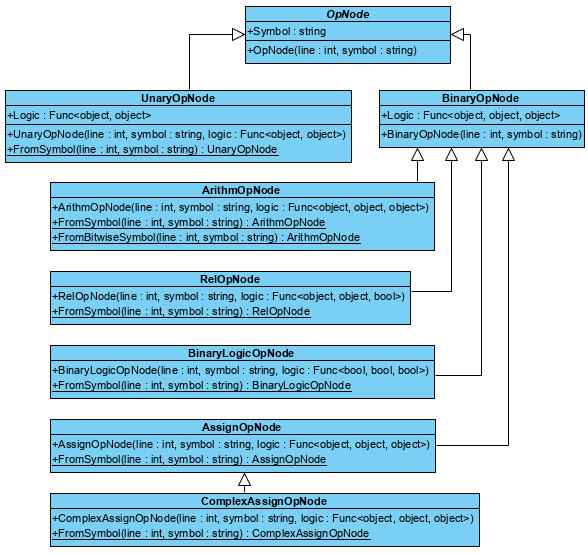
\includegraphics[scale=0.7]{images/uml/OperatorNode.png}
\caption{UML klasni dijagram (deo 1).}
\label{fig:UMLASTNode1}
\end{figure}

\begin{figure}[h!]
\centering
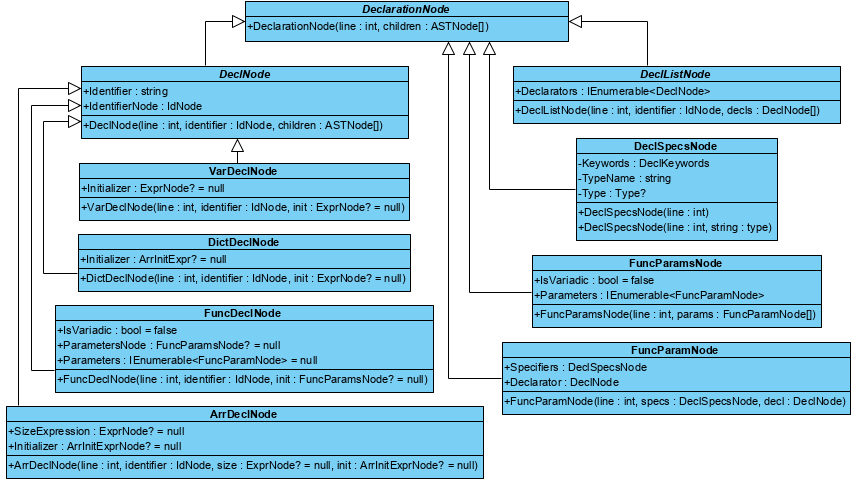
\includegraphics[scale=0.65]{images/uml/DeclarationNode.png}
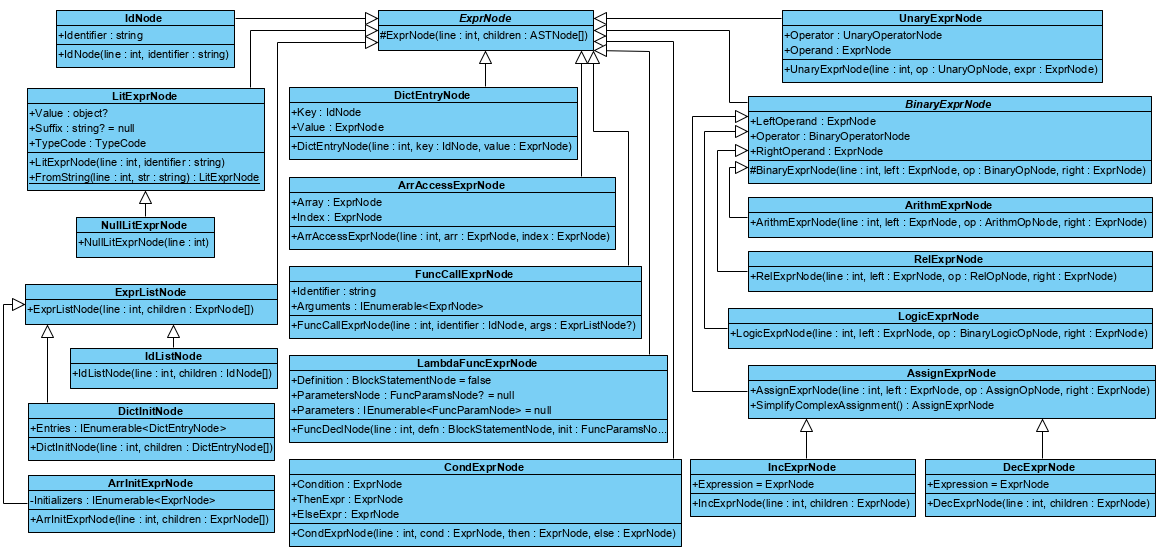
\includegraphics[scale=0.55]{images/uml/ExpressionNode.png}
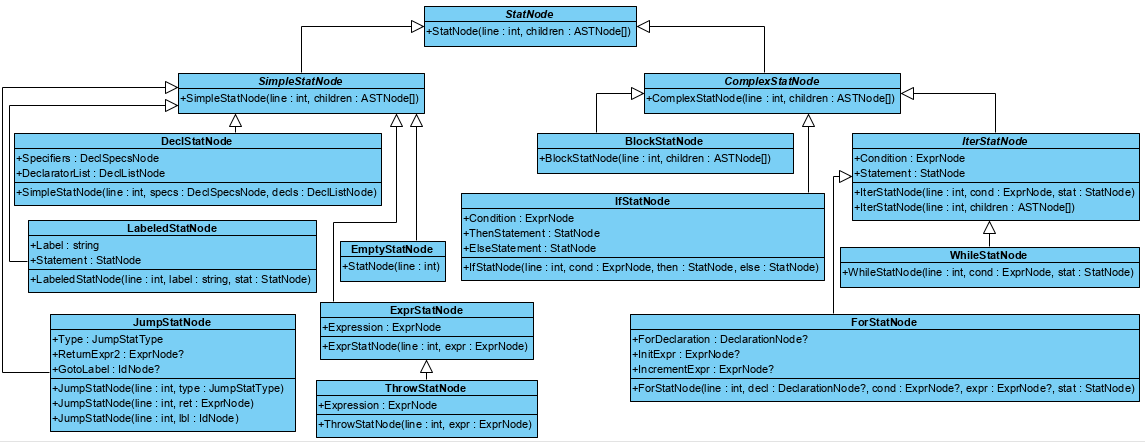
\includegraphics[scale=0.55]{images/uml/StatementNode.png}
\caption{UML klasni dijagram (deo 2).}
\label{fig:UMLASTNode2}
\end{figure}

AST struktura je \emph{imutabilna} --- ne mogu se dodavati ili uklanjati deca čvorovima. Moguće je klonirati AST čvorove ili vršiti zamenu određenog podstabla drugim podstablom ne menjajući original. Svaki AST čvor se može porediti po jednakosti sa drugim AST čvorom po intuitivnoj logici poređenja pruženom kroz predefinisane operatore poređenja.

\section{Implementacija upoređivača}
\label{sec:ImplementationComparer}

Implementacija algoritma upoređivača opisana u poglavlju \ref{chp:ASTComparing} se svodi na implementaciju funkcija za poređenje za svaki tip AST čvora. Te funkcije su enkapsulirane u klase koje implementiraju interfejs za upoređivač čvorova. Te klase nisu javne, tako da se poređenje vrši kroz upoređivač koji poredi instance tipa \texttt{ASTNode}, a koji putem refleksije određuje konkretni tip čvorova i, ukoliko su tipovi isti, pronalazi konkretni upoređivač i poziva operaciju interfejsa upoređivača. Upoređivači međusobno pozivaju jedni druge, kako bi se logika poređenja uprostila --- pošto se naredbe deklaracije sastoje od specifikatora deklaracije i liste deklaratora, upoređivač naredbi deklaracije može pozivati upoređivač za specifikatore deklaracije i upoređivač za listu deklaratora. 

Upoređivač kao rezultat svog rada vraća kolekciju potencijalnih problema (upozorenja ili grešaka) koje je detektovao prilikom analize. Ovakav pristup je odabran zbog lakoće testiranja upoređivača, s obzirom da se može očekivati određena kolekcija problema za određeni izvorni kod. Problem se modeluje kao apstraktna klasa \texttt{BaseIssue} dok se upozorenja ili greške modeluju kroz njene konkretizacije \texttt{BaseWarning} i \texttt{BaseError}. Konkretne greške, kao što su npr. nedostatak deklaracija se mogu onda modelovati kao konkretizacije ovih klasa u zavisnosti od ozbiljnosti problema. Primer izlaza upoređivača za algoritam \emph{swap} se može videti na slici \ref{fig:ComparerSwap}.

\begin{figure}[h!]
\centering
%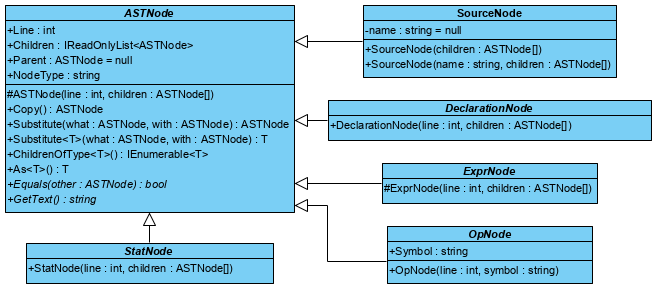
\includegraphics[scale=0.7]{images/uml/ASTNode.png}
\caption{Rezultat rada upoređivača za \texttt{swap} algoritam.}
\label{fig:ComparerSwap}
\end{figure}

\section{Implementacija vizualnog prikaza AST}
\label{sec:ImplementationVisualizer}

Osim serijalizacije AST u JSON format, kreiran je potprogram za vizualni prikaz AST-a (u daljem tekstu \emph{vizualizator}). Primeri izlaza vizualizatora se mogu videti na slikama iz poglavlja \ref{chp:MyAST} --- \ref{fig:MyASTExampleCDeclaration}, \ref{fig:MyASTExampleLuaDeclaration}, \ref{fig:MyASTExampleExpressions} i \ref{fig:MyASTExampleStatement}. Prikaz je izvršen koristeći nativni \texttt{Graphics} paket i, s obzirom da je u pitanju \emph{.NET Core 3.1} radni okvir, moguće je dobiti vizualni prikaz nezavisno od sistema.

Vizualizacija počiva na rekurzivnom algoritmu prikaza u dubinu --- za svaki čvor se prikažu potomci, rasporede jednako po širini, a onda se roditelj centrira u odnosu na ukupnu širinu koju zauzimaju deca. Ovaj pristup nije prostorno optimalan, zbog varijacija u broju dece za čvorove različitih tipova. Što se informacija za svaki čvor tiče, prikazuju se vrednosti svih atributa čvora zajedno sa njegovim tipom u zaglavlju kao i grane do njegovih potomaka.

\section{Implementacija korisničkog interfejsa}
\label{sec:ImplementationUI}

S obzirom da je aplikacija konzolna (osim komponente za vizualizaciju), korisnički interfejs se svodi na argumente komandne linije. Pokretanje programa bez argumenata pruža prikaz za pomoć u kome su nabrojane sve opcije, prikazano na slici \ref{fig:UIImpl}.

\begin{figure}[h!]
\centering
%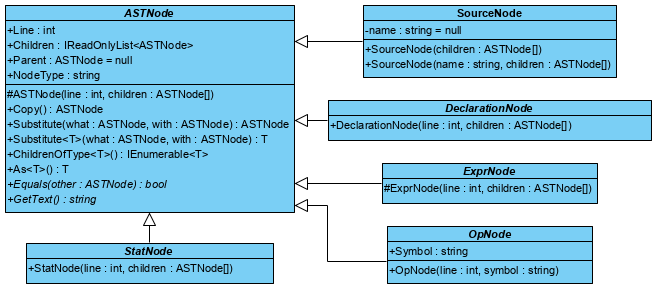
\includegraphics[scale=0.7]{images/uml/ASTNode.png}
\caption{Korisniči interfejs programa pružen kroz argumente komandne linije.}
\label{fig:UIImpl}
\end{figure}

\section{Testovi}
\label{sec:ImplementationTests}

Komponentu za kreiranje AST i komponentu za poređenje AST prate testovi jedinica koda. Testovi su organizovani u zasebnom projektu na sledeći način:
\begin{itemize}
    \item \texttt{LICC.Tests.AST} --- Testovi za adaptere i posetioce, kao i testovi funkcionalnosti metoda klase \texttt{ASTNode}.
    \item \texttt{LICC.Tests.Core} --- Testovi upoređivača.
\end{itemize}

Radni okvir koji se koristi za testiranje je \texttt{NUnit}\footnote{\url{https://nunit.org/}} koji pruža tzv. \emph{model ograničenja} (engl. \emph{constraint model}) i time omogućava pisanje čitljivog koda. Pisanje testova po modelu ograničenja se sastoji od korišćenja jednog metoda za pisanje svih testova koji kao argumente prima objekat koji se testira i složeni objekat koji predstavlja ograničenje koje objekat koji se testira treba da zadovoljava. Primer testa pisanog u ovom radnom okviru uz model ograničenja u kontekstu implementacije ovog rada se može videti na slici \ref{fig:ImplTestsUnit}.

\begin{figure}[h!]
\centering
\begin{lstlisting}
[Test]
public void ComplexDefinitionTest()
{
    FuncDefNode f = this.AssertFunctionSignature(@"
        float f(const unsigned int x, ...) {
            int z = 4;
            return 3.0;
        }", 
        2, "f", "float", isVariadic: true, 
        @params: ("unsigned int", "x")
    );
    Assert.That(f.IsVariadic);
    Assert.That(f.Definition.Children, Has.Exactly(2).Items);
}

protected FuncDefNode AssertFunctionSignature(
    string src, int line, string fname, 
    string returnType = "void", bool isVariadic = false, 
    AccessModifiers access = AccessModifiers.Unspecified,
    QualifierFlags qualifiers = QualifierFlags.None, 
    params (string Type, string Identifier)[] @params)
{
    FuncDefNode f = this.GenerateAST(src).As<FuncDefNode>();
    this.AssertChildrenParentProperties(f);
    this.AssertChildrenParentProperties(f.Definition);
    Assert.That(f, Is.Not.Null);
    Assert.That(f.Line, Is.EqualTo(line));
    Assert.That(f.Declarator, Is.Not.Null);
    Assert.That(f.Declarator.Parent, Is.EqualTo(f));
    Assert.That(f.Keywords.AccessModifiers, Is.EqualTo(access));
    Assert.That(f.Keywords.QualifierFlags, Is.EqualTo(qualifiers));
    Assert.That(f.Identifier, Is.EqualTo(fname));
    Assert.That(f.ReturnTypeName, Is.EqualTo(returnType));
    Assert.That(f.IsVariadic, Is.EqualTo(isVariadic));
    if (@params?.Any() ?? false) {
        Assert.That(f.Parameters, Is.Not.Null);
        Assert.That(f.Parameters, Has.Exactly(@params.Length).Items);
        Assert.That(f.ParametersNode, Is.Not.Null);
        Assert.That(
            f.Parameters.Select(
                p => (p.Specifiers.TypeName, p.Declarator.Identifier)
            ), 
            Is.EqualTo(@params)
        );
    }
    return f;
}
\end{lstlisting}
\caption{Primer jediničnog testa za proveru generisanog AST čvora za datu funkciju.}
\label{fig:ImplTestsUnit}
\end{figure}

Osim testova jedinica koda, prisutni su i testovi integracije svih komponenti. Kao što je opisano u prethodnim odeljcima, rezultat rada adaptera je AST, dok je rezultat data upoređivača za data dva stabla kolekcija problema. Ta dva odvojena procesa se onda mogu spojiti kako bi se testirala integracija te dve komponente --- dakle, od dva programa očekivati određenu kolekciju problema. Primer za \emph{swap} algoritam se može videti na slici \ref{fig:ImplTestsIntegration}.

\begin{figure}[h!]
\centering
\begin{lstlisting}
[Test]
public override void DifferenceTests()
{
    this.Compare(
        this.FromPseudoSource(@"
            algorithm Swap 
            begin
                declare integer x = vx
                declare integer y = vy
                procedure swap()
                begin
                    declare integer tmp = x
                    x = y  
                    y = tmp
                end
            end
        "),
        this.FromCSource(@"
            int x = vx, y = vy;
            void swap() {
                int tmp = x; y = tmp; x = y;
            }
        "),
        new MatchIssues()
            .AddError(
                new BlockEndValueMismatchError("x", 1, "vy", "vx")
            )
            .AddError(
                new BlockEndValueMismatchError("x", 3, "vy", "vx")
            )
    );
}

protected void Compare(ASTNode src, ASTNode dst, 
    MatchIssues? expectedIssues = null)
{
    expectedIssues ??= new MatchIssues();
    MatchIssues issues = new ASTNodeComparer(src, dst)
        .AttemptMatch();
    Assert.That(issues, Is.EquivallentTo(expectedIssues));
}
\end{lstlisting}
\caption{Primer kompletnog testa za algoritam \emph{swap}.}
\label{fig:ImplTestsIntegration}
\end{figure}

